	\section{Estructura básica}

		METAPESCA es un modelo general para la dinámica poblacional y pesquera de una metapoblación de organismos bentónicos, compuesta por subpoblaciones conectadas entre ellas por dispersión larval. En su versión inicial, el modelo tenía algunos aspectos en común con un modelo de simulación utilizado por Botsford (1995) y Botsford et al. (1998) para explorar la dinámica de este tipo de recursos. Esos modelos fueron discutidos en detalle durante un taller conducido en octubre de 2001 en Valparaíso, del que participó el Prof. Botsford. El y su grupo los han aplicado específicamente a los stocks de erizo de California, así como en la exploración de estrategias rotativas y de los efectos de áreas marinas protegidas. Versiones ulteriores de METAPESCA incorporan explícitamente el proceso de pesca y el manejo.
		
		
		El código del modelo está escrito en VBA (Visual Basic for Applications) utilizando EXCEL como plataforma. 

		Tiene una estructura modular, consistiendo de los siguientes módulos principales que son llamados en cada iteración desde el módulo principal:

			\begin{enumerate}
				\item Recepción de nuevos “settlers” (procesos post-dispersión) \emph{M4\_CalcRecruits}.
				\item Producción y distribución de las larvas (dispersión, introducido mediante una matriz de conectividad) \emph{M6\_Prod\_Alloc\_Larvae}
				\item Estrategias de manejo (globales, espaciales, medidas temporarias) \emph{Management\_Procedure}
				\item Asignación del esfuerzo de pesca (\emph{M7\_Fishing}).						
				\item Dinámica de cada subpoblación bentónica (crecimiento, mortalidad, etc.) \emph{M5\_Popdyn}

			\end{enumerate}

		\subsection {Recepción de nuevos “settlers”}
			Este modulo describe los procesos locales post-dispersión operando en cada celda receptora. Se encuentra contemplada la implementación de mecanismos compensatorios (inhibición del asentamiento por parte de los residentes) y depensatorios (atracción o protección de larvas competentes por parte de los residentes).

		\subsection{Producción y distribución de larvas}

			La produccion larval esta afectada por  procesos locales pre-dispersión en cada celda emisora de larvas de la matriz espacial. Estos procesos incluyen mecanismos compensatorios (denso-dependencia en el crecimiento, y por ende en el output reproductivo) y depensatorios (denso-dependencia de las tasas de fertilización). En su forma inicial la produccion de larvas asume la forma general de una función stock-reclutamiento tipo Beverton-Holt, aunque en este caso la relación no describe un proceso cerrado (como en la teoría clásica) sino la relación entre estadíos sucesivos de un proceso abierto. Este tipo de relación es esperable cuando existe un balance entre compensación y depensación pre-dispersivas; fenómenos de este tipo han sido bien documentados en el caso de los erizos (Citas).

			El proceso de dispersión larval es introducido mediante una matriz de conectividad entre las celdas. Los elementos de la matriz pueden ser especificados uno a uno por el usuario, pero se contemplan algunos prototipos básicos: subpoblaciones cerradas, conectividad a través de áreas adyacentes, pool larvario común entre subpoblaciones, y el caso en que la probabilidad de dispersión entre la celda emisora y la receptora es alguna función de la distancia entre las mismas o su posición geográfica (ESPECIFICAR TIPOS DE MODELOS, ver OKUBO). En estos casos puede especificarse la fracción de larvas retenida en cada área y el resto es distribuido automáticamente en función del prototipo de metapoblacion elegido. También existe la opción de importar la matriz de conectividad desde un archivo externo, por ejemplo archivos de salida de modelos de circulación o a través de análisis de tasas de recuperación de áreas post-explotación.

		\subsection{Estrategias de manejo}

			Las estrategias de manejo utilizadas pueden ser  tanto globales, espaciales y temporarias.
Dentro de las globales estan implementadas cuotas anuales de captura  y esfuerzo. Las medidas espaciales incluyen el uso de reservas (o refugios reproductivos) y rotacion de areas. La rotacion de areas es caracterizada a travez de la determinacion de un numero o fraccion del area total explotada y una densidad minima de reapertura de areas. Las medidas temporarias incluyen cierres por biotoxinas, proteccion de areas con juveniles, contaminacion o variaciones en la calidad del recurso. Otra medida de manejo utilizable es el uso de tallas minimas de captura.

		\subsection{Asignación del esfuerzo de pesca}

			En la implementación de estrategias de manejo espacialmente explícitas es indispensable analizar el comportamiento de asignación espacial del esfuerzo por parte de los pescadores. El análisis básico utiliza como modelos de referencia (análogos a un modelo nulo) la bien conocida Ideal Free Distribution (IFD) y la asignación proporcional (modelo gravimétrico). Se ha explorado el rango de niveles de depleción en que ambas son aproximadamente equivalentes, y se prevé en el futuro incluir otras variantes del modelo gravimétrico (Caddy, 1975, Walters et al., 1993).

			Las variantes que se prevén incorporar incluyen matrices de distancias entre subpoblaciones (o procedencias) y “puertos” (sitios de partida, desembarque, comercialización), así como los costos operativos asociados; relaciones entre calidad del recurso y precio; costos de cambiar de lugar (“switching”); “suitability” de las áreas debida a factores distintos de las distancias (dependiente de las “utility functions” percibidas por los pescadores), etc.

			En determinadas situaciones no es necesario o practico modelar el esfuerzo, como el caso de la pesqueria de Geoducks en USA donde parcelas (tracks) asignadas a pesca son explotados hasta llegar a un umbral determinado, siendo irrelevante el patron de distribucion espacial del esfuerzo requerido para llegar a dicho umbral.

		\subsection {Dinámica de cada subpoblación bentónica}

			Dinámica de las subpoblaciones, incluyendo crecimiento y mortalidad. El crecimiento está modelado de forma recursiva, de manera de poder agregar denso-dependencia. El crecimiento compensatorio esta modelado mediante una funcion lineal en funcion de la fraccion de la capacidad de carga poblacional (K) en la que se encuentra cada subpoblacion y la fraccion del alfa maximo de crecimiento.

		\subsection{Esquema general}
		
			\begin{figure}[htb]
				\begin{center}
					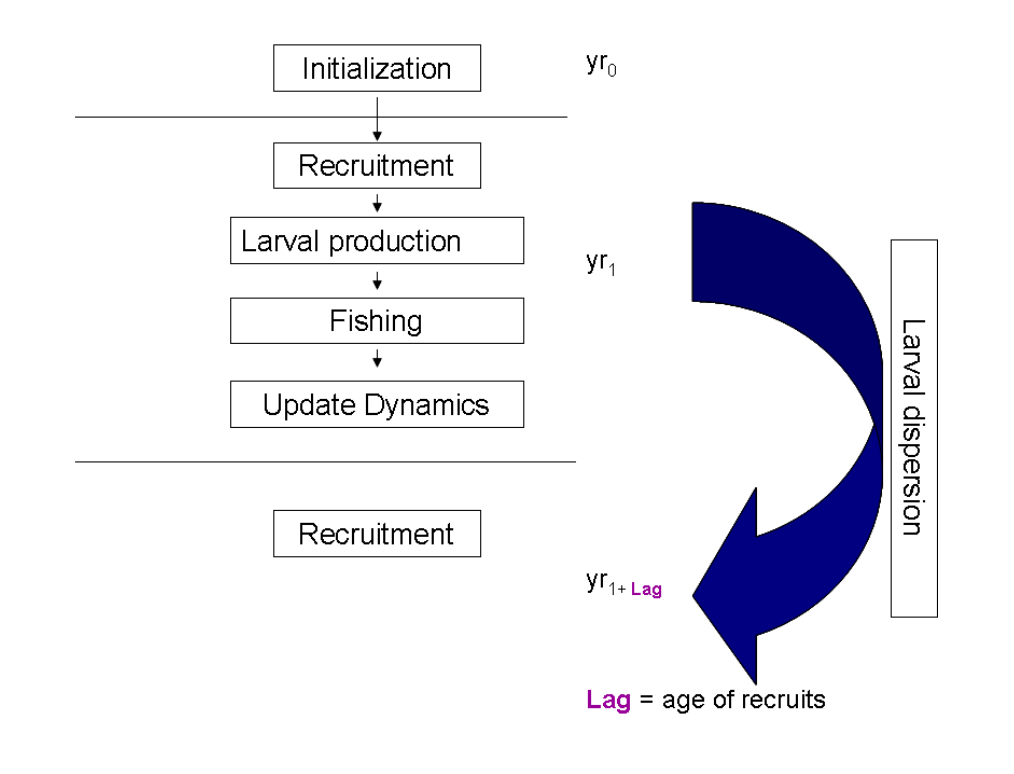
\includegraphics[width=\textwidth]{MetapescaDinamics.png}
					\caption{Esquema del orden de los eventos en el modelo.}
					\label{fig:Esquema general}
				\end{center}
			\end{figure}	
		
		El código incluye, además, módulos que agrupan la generación del output, gráficos y menús. 

		La siguientes son las principales variables de estado de la dinámica poblacional:
		\begin{enumerate}
			\item Numero de individuos a la edad, tiempo, procedencia.
			\item Talla a la edad, tiempo, procedencia.
			\item Biomasas desovante, explotable y total corregidas por variación de talla a la edad.
			\item Numero de huevos producidos por población.
			\item Numero de larvas asentándose por población.
		\end{enumerate}
 
